\subsection{Whole-section tissue mapping and neighbor retention}
\label{app:dual-view}

The tissue-mapping evaluation uses the MOSTA and HESTA held-out sections listed in Appendix~\ref{app:preprocessing}. Both atlases include cross-method comparisons and the granularity-specific No Cross comparison. ZoomST and public pretrained encoders remain frozen; target-fitted methods are identified separately.

The equal-budget controlled ablation compares the final ZoomST and No Cross checkpoints after the same total number of training updates within each atlas; No Cross omits cross-granularity supervision. Both models use the same joint readout and are frozen during evaluation. Optimization and update budgets are specified in Appendix~\ref{app:hyperparameters}.

The displayed Molecular View, Spatial View, and Joint refer to three readouts of the same frozen ZoomST model. Molecular features concatenate the three 256-dimensional outputs $e_8,e_{32},e_{128}$; spatial features concatenate $g_8,g_{32},g_{128}$. Joint features concatenate all six outputs. For MOSTA, Novae uses its public mouse-0 checkpoint; SToFM uses its public checkpoint with the declared mouse-to-human gene mapping. Each ZoomST or public pretrained candidate is independently standardized and projected to 32 dimensions using randomized PCA with seed 42, 32 oversamples, five power iterations, and no whitening. Standardization and PCA fit all eligible target-section positions without annotation values. MiniBatchKMeans uses $K$ clusters, where $K$ is the number of classes in the section's primary MOSTA \texttt{annotation} field or HESTA coarse \texttt{celltype} field, with k-means++ initialization, ten initializations, batch size 4,096, at most 300 iterations, a ten-step no-improvement limit, and seeds 42, 43, and 44.

Scores use the same eligible positions for every method within each benchmark: all positions for MOSTA and the common valid cohort specified below for the HESTA cross-method comparison. Adjusted mutual information (AMI) and adjusted Rand index (ARI) measure chance-adjusted agreement between the cluster partition and the atlas annotation. One-to-one maximum-overlap Hungarian matching assigns anatomical labels to clusters for the maps and class-specific IoU. For class $c$, $\operatorname{IoU}_c=\operatorname{TP}_c/(\operatorname{TP}_c+\operatorname{FP}_c+\operatorname{FN}_c)$. AMI and ARI are invariant to the matching. Section-level scores are averaged with equal section weights.

\paragraph{Target-fitted spatial methods.}
GraphST, BANKSY, MENDER, and STAGATE~\citep{long2023graphst,singhal2024banksy,yuan2024mender,dong2022stagate} use each complete target section independently, with expression and coordinates but no anatomical training labels. Each fixed representation uses the shared clustering protocol above. Tables group these target-fitted methods separately from frozen pretrained representations.

GraphST and STAGATE select 3,000 highly variable genes by Seurat-v3 on raw counts, followed by counts-per-10,000 normalization and log1p. GraphST additionally applies noncentered gene scaling clipped at 10. GraphST uses its Stereo-seq three-neighbor graph and a sparse implementation of the native objective, with 600 epochs, learning rate 0.001, and hidden dimension 64. The readout uses its normalized reconstructed-gene output. STAGATE uses the official PyG model, a symmetrized six-neighbor graph with self loops, hidden dimensions 512 and 30, 1,000 epochs, learning rate 0.001, weight decay 0.0001, and gradient clipping at 5. It uses the full section graph without an annotation-derived auxiliary graph.

BANKSY and MENDER normalize all genes to counts per 10,000, apply log1p, and select 3,000 genes by Seurat dispersion. BANKSY uses neighborhood statistics with 15 and 30 neighbors for orders zero and one and scaled-Gaussian decay. The fixed primary weight is $\lambda=0.8$, the official default for tissue-domain segmentation~\citep{singhal2024banksy}; the documentation explicitly includes Stereo-seq among the technologies for which this setting is recommended.\footnote{\url{https://prabhakarlab.github.io/Banksy/}, accessed 15 September 2026.} BANKSY's native channel normalization and weighting are preserved, without a second StandardScaler before PCA32. MENDER derives 32 unsupervised expression states using StandardScaler, PCA32, and MiniBatchKMeans with ten initializations; it then aggregates these states over six rings with ring parameter four, including the center, producing 192 features. MENDER's state labels are independent of the anatomical annotation.

The shared randomized-PCA and clustering settings above apply to these features. STAGATE retains its native 30 dimensions; the other methods use PCA32. The comparison shares positions, labels, and downstream algorithms while retaining these method-specific feature definitions.

\paragraph{Human cross-method benchmark.}
Table~\ref{tab:hesta-representation-summary} uses the independently pretrained human ZoomST model and seven HESTA sections. All methods share 1,129,281 positions with valid representations, excluding six positions outside the common cohort. Novae uses its public human-0 checkpoint with native count normalization, log1p, and unlabeled per-section gene selection and scaling. SToFM uses human gene names directly. scGPT-spatial normalizes raw expression by the whole-section matched nonzero mean and pretrained gene means. TERRA~\citep{birk2026terra} provides Cell, Neighborhood, and Spatial-cell outputs using its native shifted-log input, ten-neighbor context, and 2,816-token limit. These encoders use their public weights without target-section updates.

CellWorld-base~\citep{liu2026cellworld} receives raw counts normalized to 10,000 per position, followed by log1p and selection of 300 highly variable genes per section. We use Scanpy's Seurat-dispersion selection with 20 bins and no batch key. Its native tokenizer and normalized-coordinate Hilbert ordering form contexts of 4,096 positions; unknown organ and platform identifiers are set to zero. The encoder remains frozen. All native feature construction uses unlabeled section data; the common cohort and shared standardization, PCA32, and clustering readout are then applied. Public models retain their original pretraining corpora; exposure to individual HESTA target sections is not established here.

DECIPHER~\citep{xia2025decipher} is fitted independently on each target section without anatomical labels, yielding its native 32-dimensional Center and Context representations. Version 0.3.2 selects 2,000 Seurat-v3 highly variable genes from counts, normalizes to 10,000, applies log1p, and scales with clipping at 10. The minimum gene count per position is zero to retain the evaluation rows; genes require three expressing positions. The native spatial graph uses 20 neighbors. Both training stages use batch size 256, and a limit of five epochs or 10,000 updates, whichever occurs first. The molecular encoder uses a 256-unit hidden layer and learning rate 0.001; the spatial encoder uses three single-head transformer layers and learning rate 0.0001. Both use weight decay $10^{-5}$. Standardization and PCA32 precede the shared readouts.

The compact table labels Nbh., S-cell, Ctr., and Ctx. denote Neighborhood, Spatial-cell, Center, and Context, respectively. Molecular and Spatial denote the two ZoomST views defined above.

\paragraph{Whole-section anatomical results.}
Tables~\ref{tab:representation-summary} and~\ref{tab:hesta-representation-summary} report mean AMI across three downstream clustering initializations for eight MOSTA and seven HESTA sections, respectively. Table~\ref{tab:representation-secondary-ari} reports MOSTA ARI from the same runs, including sample standard deviations (denominator $3-1$). For each atlas's summary, sections are averaged equally within each clustering run before averaging the runs. Reported standard deviations quantify clustering variability with fixed representations and sections. Bold marks the top three unrounded values in each comparison, including exact third-place ties. Joint ZoomST features have the highest mean MOSTA ARI (0.345).

\begin{table}[t]
\centering\small
\caption{\textbf{ARI on all eight held-out sections.} Methods, positions, class sets, and clustering seeds match Table~\ref{tab:representation-summary}. Values are mean $\pm$ sample SD over downstream clustering initializations; the last row first averages sections equally within each seed. Bold marks the top three unrounded values per row, including third-place ties.}
\label{tab:representation-secondary-ari}
\setlength{\tabcolsep}{2.4pt}
\renewcommand{\arraystretch}{1.05}
\begin{tabular}{lccccccccc}
\toprule
 & \multicolumn{3}{c}{ZoomST views} & \multicolumn{2}{c}{Frozen pretrained} & \multicolumn{4}{c}{Target-fitted} \\
\cmidrule(lr){2-4}\cmidrule(lr){5-6}\cmidrule(lr){7-10}
Stage & Joint & \shortstack{Molecular\\View} & \shortstack{Spatial\\View} & Novae & SToFM & GraphST & BANKSY & MENDER & STAGATE \\
\midrule
E9.5 & \textbf{0.391} & 0.316 & \textbf{0.400} & 0.233 & 0.107 & \textbf{0.418} & 0.353 & 0.367 & 0.391 \\
 & {\scriptsize $\pm 0.026$} & {\scriptsize $\pm 0.012$} & {\scriptsize $\pm 0.024$} & {\scriptsize $\pm 0.016$} & {\scriptsize $\pm 0.006$} & {\scriptsize $\pm 0.025$} & {\scriptsize $\pm 0.031$} & {\scriptsize $\pm 0.016$} & {\scriptsize $\pm 0.039$} \\
\addlinespace[2pt]
E10.5 & 0.290 & 0.257 & 0.270 & 0.193 & 0.127 & \textbf{0.293} & 0.285 & \textbf{0.297} & \textbf{0.314} \\
 & {\scriptsize $\pm 0.015$} & {\scriptsize $\pm 0.017$} & {\scriptsize $\pm 0.009$} & {\scriptsize $\pm 0.003$} & {\scriptsize $\pm 0.004$} & {\scriptsize $\pm 0.027$} & {\scriptsize $\pm 0.005$} & {\scriptsize $\pm 0.006$} & {\scriptsize $\pm 0.033$} \\
\addlinespace[2pt]
E11.5 & \textbf{0.376} & \textbf{0.364} & \textbf{0.356} & 0.270 & 0.147 & 0.302 & 0.325 & 0.282 & 0.329 \\
 & {\scriptsize $\pm 0.007$} & {\scriptsize $\pm 0.004$} & {\scriptsize $\pm 0.015$} & {\scriptsize $\pm 0.012$} & {\scriptsize $\pm 0.008$} & {\scriptsize $\pm 0.026$} & {\scriptsize $\pm 0.029$} & {\scriptsize $\pm 0.001$} & {\scriptsize $\pm 0.022$} \\
\addlinespace[2pt]
E12.5 & \textbf{0.374} & \textbf{0.423} & 0.363 & 0.281 & 0.172 & 0.272 & \textbf{0.365} & 0.331 & 0.351 \\
 & {\scriptsize $\pm 0.023$} & {\scriptsize $\pm 0.009$} & {\scriptsize $\pm 0.011$} & {\scriptsize $\pm 0.006$} & {\scriptsize $\pm 0.020$} & {\scriptsize $\pm 0.027$} & {\scriptsize $\pm 0.019$} & {\scriptsize $\pm 0.018$} & {\scriptsize $\pm 0.034$} \\
\addlinespace[2pt]
E13.5 & \textbf{0.334} & 0.316 & 0.329 & 0.254 & 0.158 & 0.228 & \textbf{0.368} & \textbf{0.344} & 0.313 \\
 & {\scriptsize $\pm 0.022$} & {\scriptsize $\pm 0.015$} & {\scriptsize $\pm 0.006$} & {\scriptsize $\pm 0.009$} & {\scriptsize $\pm 0.013$} & {\scriptsize $\pm 0.052$} & {\scriptsize $\pm 0.030$} & {\scriptsize $\pm 0.012$} & {\scriptsize $\pm 0.016$} \\
\addlinespace[2pt]
E14.5 & 0.324 & \textbf{0.339} & 0.288 & 0.274 & 0.231 & 0.278 & \textbf{0.331} & 0.285 & \textbf{0.345} \\
 & {\scriptsize $\pm 0.025$} & {\scriptsize $\pm 0.030$} & {\scriptsize $\pm 0.001$} & {\scriptsize $\pm 0.015$} & {\scriptsize $\pm 0.008$} & {\scriptsize $\pm 0.035$} & {\scriptsize $\pm 0.016$} & {\scriptsize $\pm 0.026$} & {\scriptsize $\pm 0.043$} \\
\addlinespace[2pt]
E15.5 & 0.387 & \textbf{0.391} & 0.368 & 0.332 & 0.202 & 0.212 & \textbf{0.391} & \textbf{0.394} & 0.377 \\
 & {\scriptsize $\pm 0.007$} & {\scriptsize $\pm 0.037$} & {\scriptsize $\pm 0.017$} & {\scriptsize $\pm 0.002$} & {\scriptsize $\pm 0.002$} & {\scriptsize $\pm 0.004$} & {\scriptsize $\pm 0.017$} & {\scriptsize $\pm 0.019$} & {\scriptsize $\pm 0.005$} \\
\addlinespace[2pt]
E16.5 & 0.283 & 0.298 & \textbf{0.304} & 0.249 & 0.193 & 0.219 & \textbf{0.315} & 0.297 & \textbf{0.321} \\
 & {\scriptsize $\pm 0.025$} & {\scriptsize $\pm 0.013$} & {\scriptsize $\pm 0.004$} & {\scriptsize $\pm 0.008$} & {\scriptsize $\pm 0.004$} & {\scriptsize $\pm 0.013$} & {\scriptsize $\pm 0.013$} & {\scriptsize $\pm 0.044$} & {\scriptsize $\pm 0.014$} \\
\addlinespace[2pt]
Mean ARI & \textbf{0.345} & 0.338 & 0.335 & 0.261 & 0.167 & 0.278 & \textbf{0.342} & 0.325 & \textbf{0.343} \\
 & {\scriptsize $\pm 0.006$} & {\scriptsize $\pm 0.009$} & {\scriptsize $\pm 0.002$} & {\scriptsize $\pm 0.001$} & {\scriptsize $\pm 0.0005$} & {\scriptsize $\pm 0.005$} & {\scriptsize $\pm 0.008$} & {\scriptsize $\pm 0.006$} & {\scriptsize $\pm 0.004$} \\
\addlinespace[2pt]
\bottomrule
\end{tabular}

\end{table}

\paragraph{Granularity-specific anatomical ablation.}
At each $k\in\{8,32,128\}$, Joint concatenates $e_k$ and $g_k$ and uses the whole-section standardization, PCA32, and three-seed clustering protocol above. HESTA uses its coarse anatomical labels and all 1,129,287 positions across the seven sections. Both HESTA models' exported features pass through float16 and then float32 before feature preprocessing, giving them common stored precision. Table~\ref{tab:cross-granularity-ami}a reports the mean of equal-section means across the three downstream clustering runs. Section-level gains compare the models after averaging these runs within each held-out section. Table~\ref{tab:cross-granularity-ami-sections} gives these paired section means.

\begin{table}[!htbp]
\centering\small
\caption{\textbf{Joint AMI on every held-out section and granularity.} Each value averages the three downstream clustering runs; bold marks the higher unrounded value within each section--granularity pair.}
\label{tab:cross-granularity-ami-sections}
\setlength{\tabcolsep}{4pt}
\renewcommand{\arraystretch}{1.08}
\begin{tabular}{llcccccc}
\toprule
Dataset & Section (AMI) & \multicolumn{2}{c}{8} & \multicolumn{2}{c}{32} & \multicolumn{2}{c}{128} \\
 & & No Cross & ZoomST & No Cross & ZoomST & No Cross & ZoomST \\
\midrule
MOSTA & E9.5 E2S4 & 0.542 & \textbf{0.565} & \textbf{0.528} & 0.524 & \textbf{0.469} & 0.427 \\
 & E10.5 E2S1 & 0.528 & \textbf{0.552} & 0.509 & \textbf{0.536} & \textbf{0.516} & 0.510 \\
 & E11.5 E1S4 & 0.587 & \textbf{0.605} & 0.602 & \textbf{0.615} & 0.601 & \textbf{0.612} \\
 & E12.5 E2S1 & 0.607 & \textbf{0.609} & 0.595 & \textbf{0.617} & 0.601 & \textbf{0.608} \\
 & E13.5 E1S4 & 0.546 & \textbf{0.577} & 0.567 & \textbf{0.582} & 0.537 & \textbf{0.558} \\
 & E14.5 E2S2 & 0.577 & \textbf{0.582} & 0.562 & \textbf{0.573} & \textbf{0.542} & 0.540 \\
 & E15.5 E2S1 & 0.628 & \textbf{0.649} & 0.609 & \textbf{0.617} & 0.578 & \textbf{0.584} \\
 & E16.5 E2S13 & \textbf{0.541} & 0.541 & \textbf{0.521} & 0.505 & \textbf{0.468} & 0.464 \\
\midrule
HESTA & CS12-13 E1S3 & 0.518 & \textbf{0.533} & 0.535 & \textbf{0.546} & 0.509 & \textbf{0.526} \\
 & CS14-15 E2S1 & 0.570 & \textbf{0.572} & 0.574 & \textbf{0.580} & 0.518 & \textbf{0.529} \\
 & CS17 E1S9 & 0.498 & \textbf{0.513} & \textbf{0.534} & 0.520 & 0.508 & \textbf{0.512} \\
 & CS18 E1S2 & 0.533 & \textbf{0.569} & 0.559 & \textbf{0.569} & 0.553 & \textbf{0.557} \\
 & CS19 E1S1 & 0.537 & \textbf{0.552} & 0.534 & \textbf{0.553} & \textbf{0.532} & 0.528 \\
 & CS20 E1S6 & 0.564 & \textbf{0.581} & 0.577 & \textbf{0.584} & 0.564 & \textbf{0.579} \\
 & CS23 E1S3 & 0.530 & \textbf{0.561} & 0.538 & \textbf{0.550} & 0.527 & \textbf{0.531} \\
\bottomrule
\end{tabular}

\end{table}

\paragraph{Neighbor retention.}
Neighbor retention compares neighborhood membership in physical and representation spaces, describing local geometric correspondence alongside anatomical agreement.
Let $N_k^p(i)$ and $N_k^z(i)$ denote the $k$ nearest neighbors of query $i$ in physical coordinates and the corresponding PCA representation space, respectively. We report
\begin{equation}
R_k=\frac{1}{|Q|}\sum_{i\in Q}\frac{|N_k^p(i)\cap N_k^z(i)|}{k}.
\end{equation}
Each section supplies 2,048 queries equally spaced among eligible positions in original row order, with every eligible position as a candidate and the query excluded. Exact squared-Euclidean search breaks distance ties by source index. Integer-grid coordinates preserve raw spatial distances up to isometry where available; E15.5 retains the original spatial coordinates. Tables~\ref{tab:representation-summary} and~\ref{tab:hesta-representation-summary} use $k=32$ and the same standardized PCA features as each method's anatomical readout. ZoomST features use the view concatenations defined above. Figure~\ref{fig:dual-view-retention} displays all eight MOSTA sections, with colored lines connecting the same section across feature sets.

\paragraph{Whole-section maps.}
Both views contain molecular information: $e$ encodes aggregated expression over a spatial support, while $g$ also uses relative arrangement. Joint features exceed the molecular view on seven of eight section-level AMIs; their benefit over the spatial view varies by section (Table~\ref{tab:dual-view-sections}).

The E12.5 E2S1 display uses all 23,640 positions and the same 18-class \texttt{annotation} field and randomized-PCA readout as Table~\ref{tab:dual-view-sections}. Fixed seed 42 predictions are shown with one-to-one matched anatomical colors. Integer-grid coordinates are related to the raw coordinates by a distance-preserving rotation/reflection. Joint-feature IoUs for Brain and Choroid plexus are 0.402 and 0.228, respectively.

The E16.5 E2S13 Brain display uses all positions in the section, without smoothing or interpolation. Molecular features produce 504 extra and 74 missed Brain assignments; spatial features produce 60 extra and 373 missed assignments; joint features produce 77 extra and 97 missed assignments. These maps use the seed-42 run included in the three-seed quantitative evaluation.

\begin{figure}[!htb]
\centering
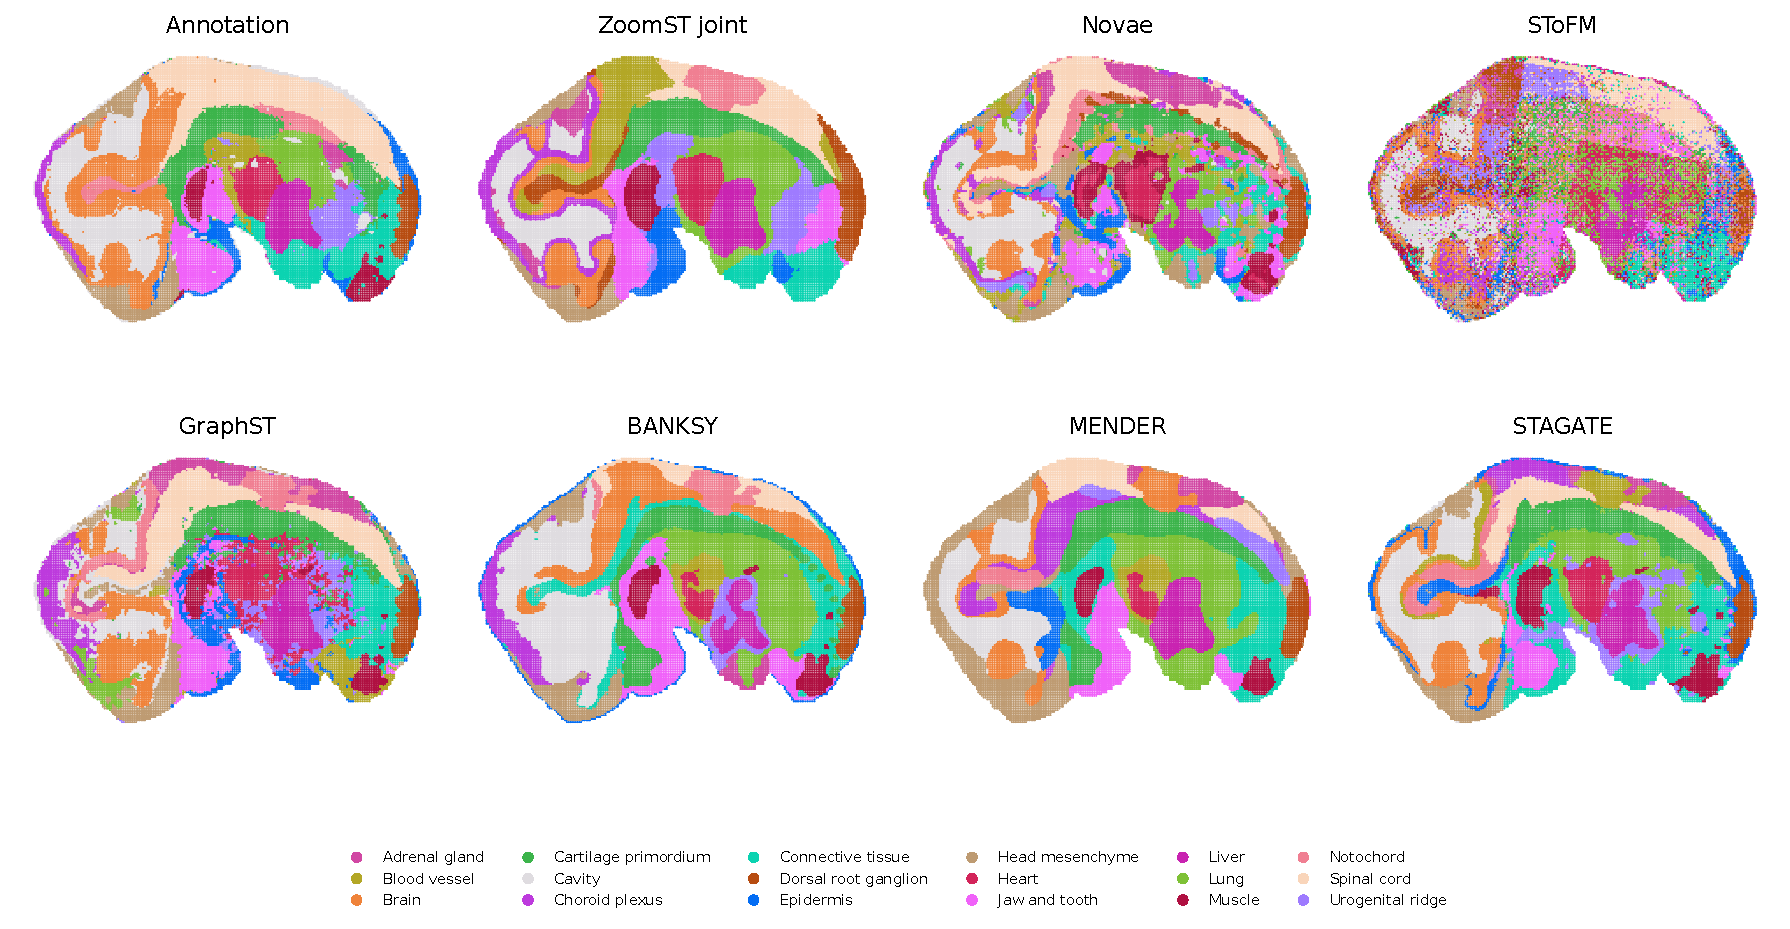
\includegraphics[width=\linewidth]{figures/e125_full_section.pdf}
\caption{\textbf{Example case: whole-section tissue mapping in E12.5 E2S1.} The annotation and seven-method predictions share all 23,640 positions and 18 primary classes. Maximum-overlap one-to-one matching assigns anatomical colors. The top row contains annotation and frozen pretrained features; the lower row contains target-fitted methods. Maps use no smoothing or label interpolation.}
\label{fig:dual-view-e125}
\end{figure}

\begin{figure}[!htbp]
\centering
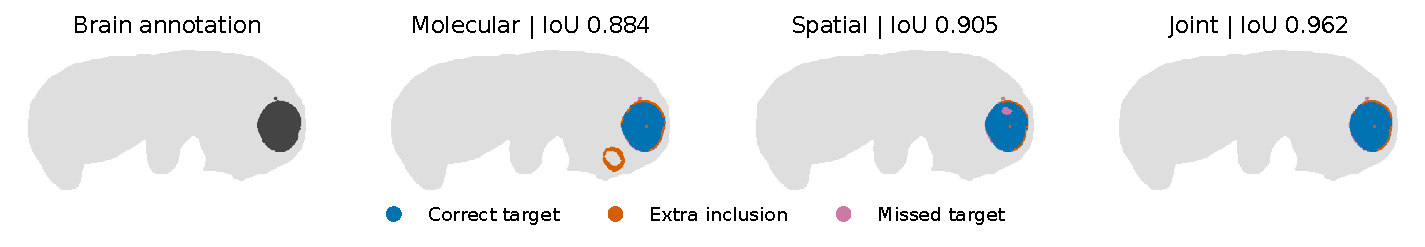
\includegraphics[width=\linewidth]{figures/brain_complementarity.pdf}
\caption{\textbf{Complementary molecular and spatial errors on a held-out section.} Annotation, molecular, spatial, and joint Brain assignments in E16.5 E2S13. Blue: correct assignments; orange: extra assignments; magenta: missed Brain.}
\label{fig:dual-view-brain}
\end{figure}

\begin{figure}[!htb]
\centering
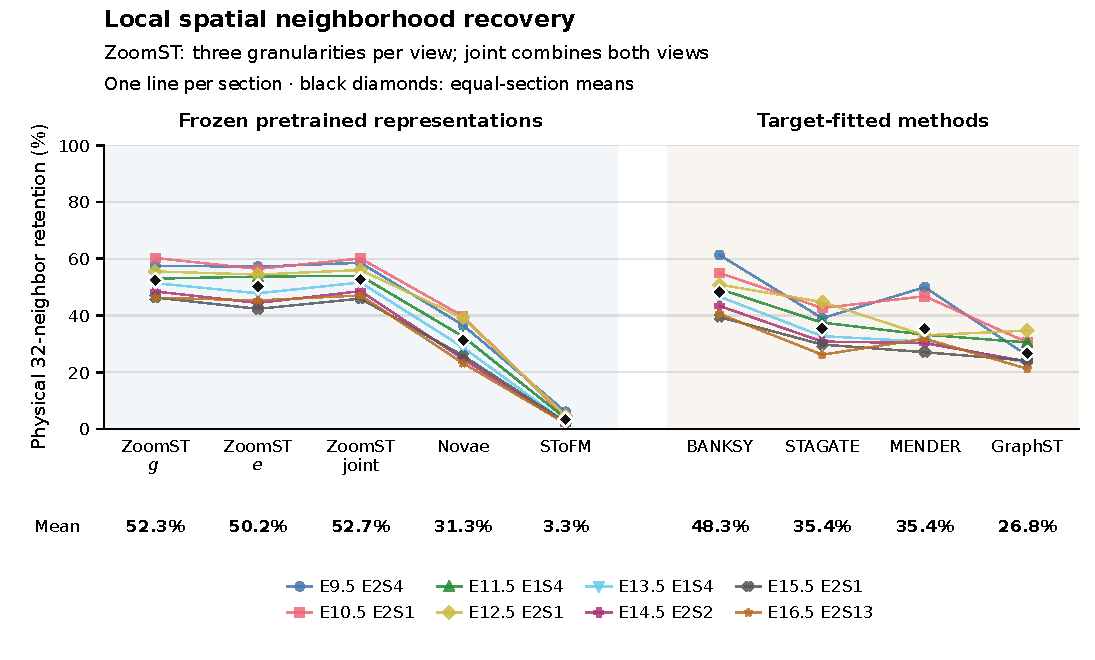
\includegraphics[width=\linewidth]{figures/spatial_retention_multiview.pdf}
\caption{\textbf{Local neighbor retention in the tissue-mapping representations.} Markers show physical 32-neighbor recovery over 2,048 fixed queries per section; all positions are candidates and self is excluded. Colored lines connect the same section within each method group, and black diamonds mark equal-section means. ZoomST $g$ and $e$ each concatenate granularities 8, 32, and 128; joint concatenates both views. All three use the same standardized PCA features as Table~\ref{tab:representation-summary}. Frozen pretrained representations and target-fitted spatial methods are grouped separately.}
\label{fig:dual-view-retention}
\end{figure}

\subsection{Developmental ordering and stage prediction within Brain}
\label{app:developmental-ordering}

MOSTA Brain is selected by coverage across all eight stages and the minimum available stage count. DPT uses the same 589 Brain observations from each held-out section, for 4,712 observations in total. HESTA Brain has sufficient coverage at CS17, CS18, CS19, CS20, and CS23; we fix 512 observations from each section, for 2,560 in total. Models share the same positions within each atlas. ZoomST and No Cross use the frozen models and Joint features defined in Appendix~\ref{app:dual-view}; the cross-method MOSTA comparison additionally uses Novae and SToFM's frozen embeddings and the shared-fit baselines below.

Table~\ref{tab:cross-granularity-development}b evaluates Joint separately at each context size $k\in\{8,32,128\}$. Within each atlas, all six model--scale combinations use the same balanced Brain cohort, 30 neighbors, and a fixed root. Each developmental stage is represented by one held-out section. Table~\ref{tab:joint-scale-comparison} additionally retains the MOSTA whole-section anatomical and physical-neighbor readouts alongside DPT.

\paragraph{Shared representations across sections.}
For the cross-method MOSTA comparison, GraphST and STAGATE each fit one encoder jointly across all eight target sections with shared gene selection and separate within-section spatial graphs. BANKSY uses a common 3,000-gene panel, and MENDER uses a common codebook of 32 unsupervised expression states. These fits use the complete target sections before extracting the balanced Brain observations. Other feature-construction and model-training settings follow Appendix~\ref{app:dual-view}.

\paragraph{Pseudotime.}
External baselines in both atlases share featurewise z-score standardization over the pooled Brain cohort, followed by PCA32 (STAGATE retains its native 30 dimensions). DPT~\citep{haghverdi2016dpt} uses Euclidean neighbor graphs and Scanpy's default distance definition with ten diffusion components.\footnote{\url{https://scanpy.readthedocs.io/en/stable/generated/scanpy.tl.dpt.html}} The default neighborhood size is 30. To address DPT computation failures, we expand the graph to 50 neighbors for STAGATE, BANKSY, and MENDER on MOSTA. Other DPT settings are shared. The MOSTA root is the E9.5 observation nearest the spatial centroid of the sampled E9.5 Brain domain. Sampling and numerical routines use seed 42. Root distances are normalized by the largest finite distance within each method; all selected MOSTA observations have finite pseudotime under the reported settings.

\paragraph{Pseudotime--stage agreement.}
For observation $i$, let $t_i$ denote pseudotime and $s_i$ its measured developmental stage. Spot-level Spearman correlation is $\operatorname{Spearman}(t_i,s_i)$ over all selected observations in an atlas, using unrounded pseudotimes and average ranks for ties. The observations span eight MOSTA stages or five HESTA stages. Figure~\ref{fig:developmental-ordering} reports both atlases; Table~\ref{tab:developmental-ordering} retains the combined-granularity MOSTA values.

For HESTA, the root is the first observation in the sorted sampled CS17 indices, fixed before evaluating the scores; its distances are normalized by the largest finite distance. ZoomST and No Cross have finite pseudotime for all selected Brain observations. Carnegie stage numbers specify the ordered target. PCA and graph construction pool the unlabeled Brain observations within each atlas; stage labels anchor the earliest-stage root and evaluate the resulting order.

\paragraph{HESTA cross-method comparison.}
The HESTA panel uses the same 2,560 Brain observations and CS17 root. Frozen external representations comprise Novae, SToFM, scGPT-spatial, the Cell, Neighborhood, and Spatial-cell outputs of TERRA, and CellWorld. They follow the standardization and DPT protocol above, with 30 neighbors for every method. CellWorld uses its frozen CP10K/log1p and per-section Seurat-HVG300 export. Its 512 CS18 observations are disconnected from the common root, so the figure marks its complete-stage readout as NA. The remaining methods cover all five stages. The existing independently fitted per-section DECIPHER embeddings are not pooled into a shared cross-stage coordinate system.

\begin{table}[!htbp]
\centering\scriptsize
\caption{\textbf{MOSTA Joint readouts by granularity.} AMI means follow Table~\ref{tab:cross-granularity-ami}a; SD is the sample SD across three downstream clustering runs. Neighbor retention is equal-section physical 32-neighbor recovery. Spot-level correlation uses the 4,712-observation Brain cohort. Bold marks the higher value in each pair, including ties.}
\label{tab:joint-scale-comparison}
\setlength{\tabcolsep}{2.2pt}
\renewcommand{\arraystretch}{1.18}
\begin{tabular}{l*{9}{c}}
\toprule
 & \multicolumn{3}{c}{AMI $\uparrow$} & \multicolumn{3}{c}{Neighbor retention (\%) $\uparrow$} & \multicolumn{3}{c}{Spot-level $\rho\uparrow$} \\
\cmidrule(lr){2-4}\cmidrule(lr){5-7}\cmidrule(lr){8-10}
Model & 8 & 32 & 128 & 8 & 32 & 128 & 8 & 32 & 128 \\
\midrule
ZoomST & \textbf{0.585 $\pm$ 0.006} & \textbf{0.571 $\pm$ 0.003} & 0.538 $\pm$ 0.002 & \textbf{35.1} & \textbf{52.7} & \textbf{62.5} & 0.868 & \textbf{0.822} & \textbf{0.354} \\
No Cross & 0.570 $\pm$ 0.001 & 0.562 $\pm$ 0.005 & \textbf{0.539 $\pm$ 0.0003} & 34.2 & 50.5 & 61.4 & \textbf{0.903} & 0.738 & -0.239 \\
\bottomrule
\end{tabular}

\end{table}

\begin{table}[!htbp]
\centering\small
\caption{\textbf{Spot-level pseudotime--stage Spearman correlation within Brain.} Correlation is computed over all 4,712 observations spanning eight MOSTA stages. Bold marks the highest value.}
\label{tab:developmental-ordering}
\setlength{\tabcolsep}{10pt}
\renewcommand{\arraystretch}{1.05}
\begin{tabular}{lc}
\toprule
Representation & \shortstack{Spot-level\\Spearman $\rho$} \\
\midrule
ZoomST joint & \textbf{0.816} \\
Novae & 0.714 \\
SToFM & 0.341 \\
ZoomST no cross & 0.651 \\
GraphST & 0.491 \\
STAGATE & 0.229 \\
BANKSY & -0.267 \\
MENDER & 0.458 \\
\bottomrule
\end{tabular}

\end{table}

\paragraph{Developmental-stage prediction.}
The linear probe uses the original Joint features without PCA. Each leave-one-section-out fold fits StandardScaler and a Ridge regressor only on Brain observations from the remaining sections. The intercept is unpenalized and the Ridge coefficient is $\alpha=n_{\mathrm{train}}\lambda$, with fixed $\lambda=0.1$. MOSTA training folds use 512 Brain observations per section and evaluate every Brain observation in the test section. HESTA uses the same fixed 512-observation-per-section cohort for training and testing across folds. Targets are embryonic days for MOSTA and Carnegie stages for HESTA. Encoder weights remain frozen throughout.

For section $s$ with $n_s$ evaluated observations, $\mathrm{MAE}_s=n_s^{-1}\sum_i|\hat{s}_i-s|$; reported MAE averages the included sections equally. Relative reduction is $(\overline{\mathrm{MAE}}_{\mathrm{No\ Cross}}-\overline{\mathrm{MAE}}_{\mathrm{ZoomST}})/\overline{\mathrm{MAE}}_{\mathrm{No\ Cross}}$.
\FloatBarrier
